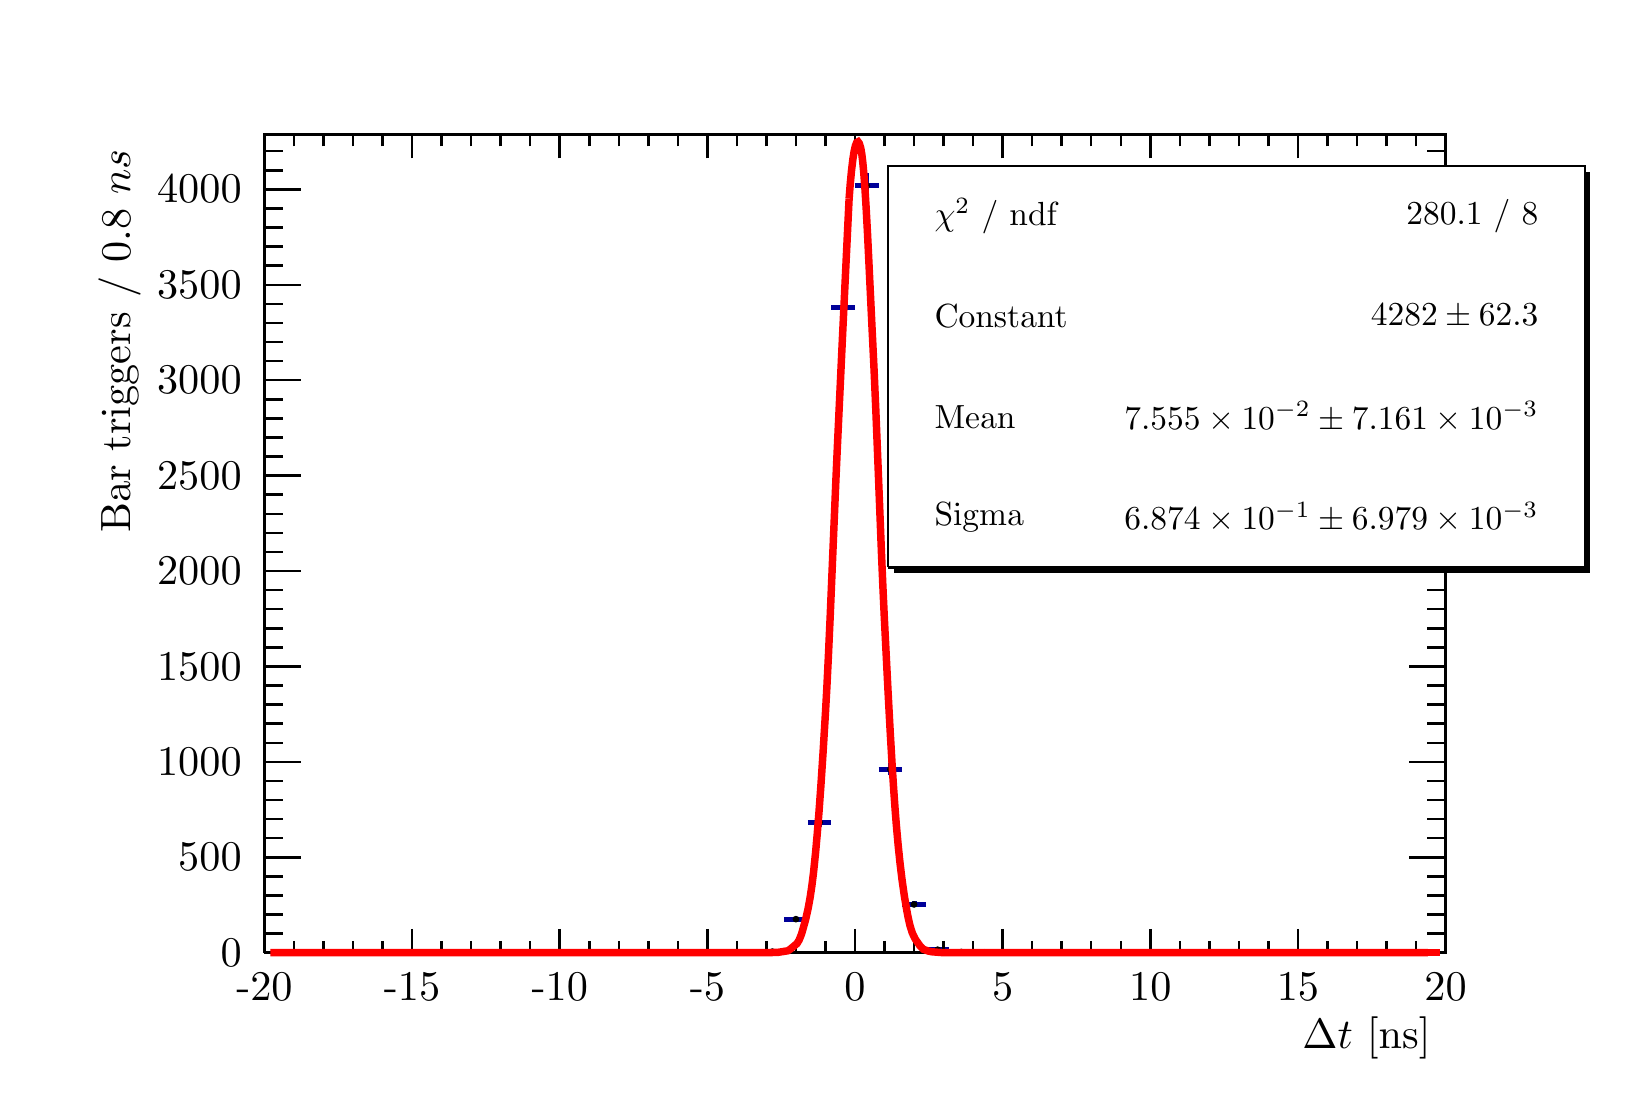
\begin{tikzpicture}
\pgfdeclareplotmark{cross} {
\pgfpathmoveto{\pgfpoint{-0.3\pgfplotmarksize}{\pgfplotmarksize}}
\pgfpathlineto{\pgfpoint{+0.3\pgfplotmarksize}{\pgfplotmarksize}}
\pgfpathlineto{\pgfpoint{+0.3\pgfplotmarksize}{0.3\pgfplotmarksize}}
\pgfpathlineto{\pgfpoint{+1\pgfplotmarksize}{0.3\pgfplotmarksize}}
\pgfpathlineto{\pgfpoint{+1\pgfplotmarksize}{-0.3\pgfplotmarksize}}
\pgfpathlineto{\pgfpoint{+0.3\pgfplotmarksize}{-0.3\pgfplotmarksize}}
\pgfpathlineto{\pgfpoint{+0.3\pgfplotmarksize}{-1.\pgfplotmarksize}}
\pgfpathlineto{\pgfpoint{-0.3\pgfplotmarksize}{-1.\pgfplotmarksize}}
\pgfpathlineto{\pgfpoint{-0.3\pgfplotmarksize}{-0.3\pgfplotmarksize}}
\pgfpathlineto{\pgfpoint{-1.\pgfplotmarksize}{-0.3\pgfplotmarksize}}
\pgfpathlineto{\pgfpoint{-1.\pgfplotmarksize}{0.3\pgfplotmarksize}}
\pgfpathlineto{\pgfpoint{-0.3\pgfplotmarksize}{0.3\pgfplotmarksize}}
\pgfpathclose
\pgfusepathqstroke
}
\pgfdeclareplotmark{cross*} {
\pgfpathmoveto{\pgfpoint{-0.3\pgfplotmarksize}{\pgfplotmarksize}}
\pgfpathlineto{\pgfpoint{+0.3\pgfplotmarksize}{\pgfplotmarksize}}
\pgfpathlineto{\pgfpoint{+0.3\pgfplotmarksize}{0.3\pgfplotmarksize}}
\pgfpathlineto{\pgfpoint{+1\pgfplotmarksize}{0.3\pgfplotmarksize}}
\pgfpathlineto{\pgfpoint{+1\pgfplotmarksize}{-0.3\pgfplotmarksize}}
\pgfpathlineto{\pgfpoint{+0.3\pgfplotmarksize}{-0.3\pgfplotmarksize}}
\pgfpathlineto{\pgfpoint{+0.3\pgfplotmarksize}{-1.\pgfplotmarksize}}
\pgfpathlineto{\pgfpoint{-0.3\pgfplotmarksize}{-1.\pgfplotmarksize}}
\pgfpathlineto{\pgfpoint{-0.3\pgfplotmarksize}{-0.3\pgfplotmarksize}}
\pgfpathlineto{\pgfpoint{-1.\pgfplotmarksize}{-0.3\pgfplotmarksize}}
\pgfpathlineto{\pgfpoint{-1.\pgfplotmarksize}{0.3\pgfplotmarksize}}
\pgfpathlineto{\pgfpoint{-0.3\pgfplotmarksize}{0.3\pgfplotmarksize}}
\pgfpathclose
\pgfusepathqfillstroke
}
\pgfdeclareplotmark{newstar} {
\pgfpathmoveto{\pgfqpoint{0pt}{\pgfplotmarksize}}
\pgfpathlineto{\pgfqpointpolar{44}{0.5\pgfplotmarksize}}
\pgfpathlineto{\pgfqpointpolar{18}{\pgfplotmarksize}}
\pgfpathlineto{\pgfqpointpolar{-20}{0.5\pgfplotmarksize}}
\pgfpathlineto{\pgfqpointpolar{-54}{\pgfplotmarksize}}
\pgfpathlineto{\pgfqpointpolar{-90}{0.5\pgfplotmarksize}}
\pgfpathlineto{\pgfqpointpolar{234}{\pgfplotmarksize}}
\pgfpathlineto{\pgfqpointpolar{198}{0.5\pgfplotmarksize}}
\pgfpathlineto{\pgfqpointpolar{162}{\pgfplotmarksize}}
\pgfpathlineto{\pgfqpointpolar{134}{0.5\pgfplotmarksize}}
\pgfpathclose
\pgfusepathqstroke
}
\pgfdeclareplotmark{newstar*} {
\pgfpathmoveto{\pgfqpoint{0pt}{\pgfplotmarksize}}
\pgfpathlineto{\pgfqpointpolar{44}{0.5\pgfplotmarksize}}
\pgfpathlineto{\pgfqpointpolar{18}{\pgfplotmarksize}}
\pgfpathlineto{\pgfqpointpolar{-20}{0.5\pgfplotmarksize}}
\pgfpathlineto{\pgfqpointpolar{-54}{\pgfplotmarksize}}
\pgfpathlineto{\pgfqpointpolar{-90}{0.5\pgfplotmarksize}}
\pgfpathlineto{\pgfqpointpolar{234}{\pgfplotmarksize}}
\pgfpathlineto{\pgfqpointpolar{198}{0.5\pgfplotmarksize}}
\pgfpathlineto{\pgfqpointpolar{162}{\pgfplotmarksize}}
\pgfpathlineto{\pgfqpointpolar{134}{0.5\pgfplotmarksize}}
\pgfpathclose
\pgfusepathqfillstroke
}
\definecolor{c}{rgb}{1,1,1};
\draw [color=c, fill=c] (0,0) rectangle (20,13.4957);
\draw [color=c, fill=c] (3,1.75444) rectangle (18,12.1461);
\definecolor{c}{rgb}{0,0,0};
\draw [c,line width=0.9] (3,1.75444) -- (3,12.1461) -- (18,12.1461) -- (18,1.75444) -- (3,1.75444);
\definecolor{c}{rgb}{1,1,1};
\draw [color=c, fill=c] (3,1.75444) rectangle (18,12.1461);
\definecolor{c}{rgb}{0,0,0};
\draw [c,line width=0.9] (3,1.75444) -- (3,12.1461) -- (18,12.1461) -- (18,1.75444) -- (3,1.75444);
\definecolor{c}{rgb}{0,0,0.6};
\draw [c,line width=1.8] (9.45,1.76305) -- (9.45,1.76898);
\draw [c,line width=1.8] (9.45,1.76898) -- (9.45,1.77492);
\draw [c,line width=1.8] (9.3,1.76898) -- (9.45,1.76898);
\draw [c,line width=1.8] (9.45,1.76898) -- (9.6,1.76898);
\definecolor{c}{rgb}{0,0,0};
\foreach \P in {(9.45,1.76898)}{\draw[mark options={color=c,fill=c},mark size=2.402402pt,mark=*,mark size=1pt] plot coordinates {\P};}
\definecolor{c}{rgb}{0,0,0.6};
\draw [c,line width=1.8] (9.75,2.14885) -- (9.75,2.18101);
\draw [c,line width=1.8] (9.75,2.18101) -- (9.75,2.21316);
\draw [c,line width=1.8] (9.6,2.18101) -- (9.75,2.18101);
\draw [c,line width=1.8] (9.75,2.18101) -- (9.9,2.18101);
\definecolor{c}{rgb}{0,0,0};
\foreach \P in {(9.75,2.18101)}{\draw[mark options={color=c,fill=c},mark size=2.402402pt,mark=*,mark size=1pt] plot coordinates {\P};}
\definecolor{c}{rgb}{0,0,0.6};
\draw [c,line width=1.8] (10.05,3.34647) -- (10.05,3.40981);
\draw [c,line width=1.8] (10.05,3.40981) -- (10.05,3.47315);
\draw [c,line width=1.8] (9.9,3.40981) -- (10.05,3.40981);
\draw [c,line width=1.8] (10.05,3.40981) -- (10.2,3.40981);
\definecolor{c}{rgb}{0,0,0};
\foreach \P in {(10.05,3.40981)}{\draw[mark options={color=c,fill=c},mark size=2.402402pt,mark=*,mark size=1pt] plot coordinates {\P};}
\definecolor{c}{rgb}{0,0,0.6};
\draw [c,line width=1.8] (10.35,9.80556) -- (10.35,9.94647);
\draw [c,line width=1.8] (10.35,9.94647) -- (10.35,10.0874);
\draw [c,line width=1.8] (10.2,9.94647) -- (10.35,9.94647);
\draw [c,line width=1.8] (10.35,9.94647) -- (10.5,9.94647);
\definecolor{c}{rgb}{0,0,0};
\foreach \P in {(10.35,9.94647)}{\draw[mark options={color=c,fill=c},mark size=2.402402pt,mark=*,mark size=1pt] plot coordinates {\P};}
\definecolor{c}{rgb}{0,0,0.6};
\draw [c,line width=1.8] (10.65,11.344) -- (10.65,11.4976);
\draw [c,line width=1.8] (10.65,11.4976) -- (10.65,11.6513);
\draw [c,line width=1.8] (10.5,11.4976) -- (10.65,11.4976);
\draw [c,line width=1.8] (10.65,11.4976) -- (10.8,11.4976);
\definecolor{c}{rgb}{0,0,0};
\foreach \P in {(10.65,11.4976)}{\draw[mark options={color=c,fill=c},mark size=2.402402pt,mark=*,mark size=1pt] plot coordinates {\P};}
\definecolor{c}{rgb}{0,0,0.6};
\draw [c,line width=1.8] (10.95,4.00846) -- (10.95,4.08359);
\draw [c,line width=1.8] (10.95,4.08359) -- (10.95,4.15873);
\draw [c,line width=1.8] (10.8,4.08359) -- (10.95,4.08359);
\draw [c,line width=1.8] (10.95,4.08359) -- (11.1,4.08359);
\definecolor{c}{rgb}{0,0,0};
\foreach \P in {(10.95,4.08359)}{\draw[mark options={color=c,fill=c},mark size=2.402402pt,mark=*,mark size=1pt] plot coordinates {\P};}
\definecolor{c}{rgb}{0,0,0.6};
\draw [c,line width=1.8] (11.25,2.32908) -- (11.25,2.36763);
\draw [c,line width=1.8] (11.25,2.36763) -- (11.25,2.40618);
\draw [c,line width=1.8] (11.1,2.36763) -- (11.25,2.36763);
\draw [c,line width=1.8] (11.25,2.36763) -- (11.4,2.36763);
\definecolor{c}{rgb}{0,0,0};
\foreach \P in {(11.25,2.36763)}{\draw[mark options={color=c,fill=c},mark size=2.402402pt,mark=*,mark size=1pt] plot coordinates {\P};}
\definecolor{c}{rgb}{0,0,0.6};
\draw [c,line width=1.8] (11.55,1.78353) -- (11.55,1.79322);
\draw [c,line width=1.8] (11.55,1.79322) -- (11.55,1.80291);
\draw [c,line width=1.8] (11.4,1.79322) -- (11.55,1.79322);
\draw [c,line width=1.8] (11.55,1.79322) -- (11.7,1.79322);
\definecolor{c}{rgb}{0,0,0};
\foreach \P in {(11.55,1.79322)}{\draw[mark options={color=c,fill=c},mark size=2.402402pt,mark=*,mark size=1pt] plot coordinates {\P};}
\definecolor{c}{rgb}{0,0,0.6};
\draw [c,line width=1.8] (11.85,1.75929) -- (11.85,1.76414);
\draw [c,line width=1.8] (11.85,1.76414) -- (11.85,1.76898);
\draw [c,line width=1.8] (11.7,1.76414) -- (11.85,1.76414);
\draw [c,line width=1.8] (11.85,1.76414) -- (12,1.76414);
\definecolor{c}{rgb}{0,0,0};
\foreach \P in {(11.85,1.76414)}{\draw[mark options={color=c,fill=c},mark size=2.402402pt,mark=*,mark size=1pt] plot coordinates {\P};}
\definecolor{c}{rgb}{0,0,0.6};
\draw [c,line width=1.8] (12.15,1.75586) -- (12.15,1.75929);
\draw [c,line width=1.8] (12.15,1.75929) -- (12.15,1.76272);
\draw [c,line width=1.8] (12,1.75929) -- (12.15,1.75929);
\draw [c,line width=1.8] (12.15,1.75929) -- (12.3,1.75929);
\definecolor{c}{rgb}{0,0,0};
\foreach \P in {(12.15,1.75929)}{\draw[mark options={color=c,fill=c},mark size=2.402402pt,mark=*,mark size=1pt] plot coordinates {\P};}
\definecolor{c}{rgb}{0,0,0.6};
\draw [c,line width=1.8] (12.45,1.75444) -- (12.45,1.75686);
\draw [c,line width=1.8] (12.45,1.75686) -- (12.45,1.75929);
\draw [c,line width=1.8] (12.3,1.75686) -- (12.45,1.75686);
\draw [c,line width=1.8] (12.45,1.75686) -- (12.6,1.75686);
\definecolor{c}{rgb}{0,0,0};
\foreach \P in {(12.45,1.75686)}{\draw[mark options={color=c,fill=c},mark size=2.402402pt,mark=*,mark size=1pt] plot coordinates {\P};}
\definecolor{c}{rgb}{1,1,1};
\draw [color=c, fill=c] (10.9169,6.64756) rectangle (19.7708,11.7479);
\definecolor{c}{rgb}{0,0,0};
\draw [c, fill=c] (11.0029,6.64756) -- (11.0029,6.59026) -- (19.8281,6.59026) -- (19.8281,11.6619) -- (19.7708,11.6619) -- (19.7708,6.64756);
\draw [c,line width=0.9] (10.9169,6.64756) -- (10.9169,11.7479) -- (19.7708,11.7479) -- (19.7708,6.64756) -- (10.9169,6.64756);
\draw [anchor= west] (11.3596,11.1103) node[scale=1.20912, color=c, rotate=0]{$\chi^{2} / ndf $};
\draw [anchor= east] (19.3281,11.1103) node[scale=1.20912, color=c, rotate=0]{ 280.1 / 8};
\draw [anchor= west] (11.3596,9.83524) node[scale=1.20912, color=c, rotate=0]{Constant };
\draw [anchor= east] (19.3281,9.83524) node[scale=1.20912, color=c, rotate=0]{$  4282 \pm 62.3$};
\draw [anchor= west] (11.3596,8.56017) node[scale=1.20912, color=c, rotate=0]{Mean     };
\draw [anchor= east] (19.3281,8.56017) node[scale=1.20912, color=c, rotate=0]{$ 7.555e-11 \pm 7.161e-12$};
\draw [anchor= west] (11.3596,7.2851) node[scale=1.20912, color=c, rotate=0]{Sigma    };
\draw [anchor= east] (19.3281,7.2851) node[scale=1.20912, color=c, rotate=0]{$ 6.874e-10 \pm 6.979e-12$};
\draw [c,line width=0.9] (3,1.75444) -- (18,1.75444);
\draw [c,line width=0.9] (3,2.05809) -- (3,1.75444);
\draw [c,line width=0.9] (3.375,1.90627) -- (3.375,1.75444);
\draw [c,line width=0.9] (3.75,1.90627) -- (3.75,1.75444);
\draw [c,line width=0.9] (4.125,1.90627) -- (4.125,1.75444);
\draw [c,line width=0.9] (4.5,1.90627) -- (4.5,1.75444);
\draw [c,line width=0.9] (4.875,2.05809) -- (4.875,1.75444);
\draw [c,line width=0.9] (5.25,1.90627) -- (5.25,1.75444);
\draw [c,line width=0.9] (5.625,1.90627) -- (5.625,1.75444);
\draw [c,line width=0.9] (6,1.90627) -- (6,1.75444);
\draw [c,line width=0.9] (6.375,1.90627) -- (6.375,1.75444);
\draw [c,line width=0.9] (6.75,2.05809) -- (6.75,1.75444);
\draw [c,line width=0.9] (7.125,1.90627) -- (7.125,1.75444);
\draw [c,line width=0.9] (7.5,1.90627) -- (7.5,1.75444);
\draw [c,line width=0.9] (7.875,1.90627) -- (7.875,1.75444);
\draw [c,line width=0.9] (8.25,1.90627) -- (8.25,1.75444);
\draw [c,line width=0.9] (8.625,2.05809) -- (8.625,1.75444);
\draw [c,line width=0.9] (9,1.90627) -- (9,1.75444);
\draw [c,line width=0.9] (9.375,1.90627) -- (9.375,1.75444);
\draw [c,line width=0.9] (9.75,1.90627) -- (9.75,1.75444);
\draw [c,line width=0.9] (10.125,1.90627) -- (10.125,1.75444);
\draw [c,line width=0.9] (10.5,2.05809) -- (10.5,1.75444);
\draw [c,line width=0.9] (10.875,1.90627) -- (10.875,1.75444);
\draw [c,line width=0.9] (11.25,1.90627) -- (11.25,1.75444);
\draw [c,line width=0.9] (11.625,1.90627) -- (11.625,1.75444);
\draw [c,line width=0.9] (12,1.90627) -- (12,1.75444);
\draw [c,line width=0.9] (12.375,2.05809) -- (12.375,1.75444);
\draw [c,line width=0.9] (12.75,1.90627) -- (12.75,1.75444);
\draw [c,line width=0.9] (13.125,1.90627) -- (13.125,1.75444);
\draw [c,line width=0.9] (13.5,1.90627) -- (13.5,1.75444);
\draw [c,line width=0.9] (13.875,1.90627) -- (13.875,1.75444);
\draw [c,line width=0.9] (14.25,2.05809) -- (14.25,1.75444);
\draw [c,line width=0.9] (14.625,1.90627) -- (14.625,1.75444);
\draw [c,line width=0.9] (15,1.90627) -- (15,1.75444);
\draw [c,line width=0.9] (15.375,1.90627) -- (15.375,1.75444);
\draw [c,line width=0.9] (15.75,1.90627) -- (15.75,1.75444);
\draw [c,line width=0.9] (16.125,2.05809) -- (16.125,1.75444);
\draw [c,line width=0.9] (16.5,1.90627) -- (16.5,1.75444);
\draw [c,line width=0.9] (16.875,1.90627) -- (16.875,1.75444);
\draw [c,line width=0.9] (17.25,1.90627) -- (17.25,1.75444);
\draw [c,line width=0.9] (17.625,1.90627) -- (17.625,1.75444);
\draw [c,line width=0.9] (18,2.05809) -- (18,1.75444);
\draw [anchor=base] (3,1.14713) node[scale=1.52731, color=c, rotate=0]{-20};
\draw [anchor=base] (4.875,1.14713) node[scale=1.52731, color=c, rotate=0]{-15};
\draw [anchor=base] (6.75,1.14713) node[scale=1.52731, color=c, rotate=0]{-10};
\draw [anchor=base] (8.625,1.14713) node[scale=1.52731, color=c, rotate=0]{-5};
\draw [anchor=base] (10.5,1.14713) node[scale=1.52731, color=c, rotate=0]{0};
\draw [anchor=base] (12.375,1.14713) node[scale=1.52731, color=c, rotate=0]{5};
\draw [anchor=base] (14.25,1.14713) node[scale=1.52731, color=c, rotate=0]{10};
\draw [anchor=base] (16.125,1.14713) node[scale=1.52731, color=c, rotate=0]{15};
\draw [anchor=base] (18,1.14713) node[scale=1.52731, color=c, rotate=0]{20};
%\draw [anchor=base west] (18.1,1.75444) node[scale=1.52731, color=c, rotate=0]{$\times10^{-9}$};
\draw [anchor= east] (18,0.674785) node[scale=1.52731, color=c, rotate=0]{$\Delta t$ [ns]};
\draw [c,line width=0.9] (3,12.1461) -- (18,12.1461);
\draw [c,line width=0.9] (3,11.8425) -- (3,12.1461);
\draw [c,line width=0.9] (3.375,11.9943) -- (3.375,12.1461);
\draw [c,line width=0.9] (3.75,11.9943) -- (3.75,12.1461);
\draw [c,line width=0.9] (4.125,11.9943) -- (4.125,12.1461);
\draw [c,line width=0.9] (4.5,11.9943) -- (4.5,12.1461);
\draw [c,line width=0.9] (4.875,11.8425) -- (4.875,12.1461);
\draw [c,line width=0.9] (5.25,11.9943) -- (5.25,12.1461);
\draw [c,line width=0.9] (5.625,11.9943) -- (5.625,12.1461);
\draw [c,line width=0.9] (6,11.9943) -- (6,12.1461);
\draw [c,line width=0.9] (6.375,11.9943) -- (6.375,12.1461);
\draw [c,line width=0.9] (6.75,11.8425) -- (6.75,12.1461);
\draw [c,line width=0.9] (7.125,11.9943) -- (7.125,12.1461);
\draw [c,line width=0.9] (7.5,11.9943) -- (7.5,12.1461);
\draw [c,line width=0.9] (7.875,11.9943) -- (7.875,12.1461);
\draw [c,line width=0.9] (8.25,11.9943) -- (8.25,12.1461);
\draw [c,line width=0.9] (8.625,11.8425) -- (8.625,12.1461);
\draw [c,line width=0.9] (9,11.9943) -- (9,12.1461);
\draw [c,line width=0.9] (9.375,11.9943) -- (9.375,12.1461);
\draw [c,line width=0.9] (9.75,11.9943) -- (9.75,12.1461);
\draw [c,line width=0.9] (10.125,11.9943) -- (10.125,12.1461);
\draw [c,line width=0.9] (10.5,11.8425) -- (10.5,12.1461);
\draw [c,line width=0.9] (10.875,11.9943) -- (10.875,12.1461);
\draw [c,line width=0.9] (11.25,11.9943) -- (11.25,12.1461);
\draw [c,line width=0.9] (11.625,11.9943) -- (11.625,12.1461);
\draw [c,line width=0.9] (12,11.9943) -- (12,12.1461);
\draw [c,line width=0.9] (12.375,11.8425) -- (12.375,12.1461);
\draw [c,line width=0.9] (12.75,11.9943) -- (12.75,12.1461);
\draw [c,line width=0.9] (13.125,11.9943) -- (13.125,12.1461);
\draw [c,line width=0.9] (13.5,11.9943) -- (13.5,12.1461);
\draw [c,line width=0.9] (13.875,11.9943) -- (13.875,12.1461);
\draw [c,line width=0.9] (14.25,11.8425) -- (14.25,12.1461);
\draw [c,line width=0.9] (14.625,11.9943) -- (14.625,12.1461);
\draw [c,line width=0.9] (15,11.9943) -- (15,12.1461);
\draw [c,line width=0.9] (15.375,11.9943) -- (15.375,12.1461);
\draw [c,line width=0.9] (15.75,11.9943) -- (15.75,12.1461);
\draw [c,line width=0.9] (16.125,11.8425) -- (16.125,12.1461);
\draw [c,line width=0.9] (16.5,11.9943) -- (16.5,12.1461);
\draw [c,line width=0.9] (16.875,11.9943) -- (16.875,12.1461);
\draw [c,line width=0.9] (17.25,11.9943) -- (17.25,12.1461);
\draw [c,line width=0.9] (17.625,11.9943) -- (17.625,12.1461);
\draw [c,line width=0.9] (18,11.8425) -- (18,12.1461);
\draw [c,line width=0.9] (3,1.75444) -- (3,12.1461);
\draw [c,line width=0.9] (3.462,1.75444) -- (3,1.75444);
\draw [c,line width=0.9] (3.231,1.99681) -- (3,1.99681);
\draw [c,line width=0.9] (3.231,2.23918) -- (3,2.23918);
\draw [c,line width=0.9] (3.231,2.48154) -- (3,2.48154);
\draw [c,line width=0.9] (3.231,2.72391) -- (3,2.72391);
\draw [c,line width=0.9] (3.462,2.96628) -- (3,2.96628);
\draw [c,line width=0.9] (3.231,3.20865) -- (3,3.20865);
\draw [c,line width=0.9] (3.231,3.45101) -- (3,3.45101);
\draw [c,line width=0.9] (3.231,3.69338) -- (3,3.69338);
\draw [c,line width=0.9] (3.231,3.93575) -- (3,3.93575);
\draw [c,line width=0.9] (3.462,4.17812) -- (3,4.17812);
\draw [c,line width=0.9] (3.231,4.42049) -- (3,4.42049);
\draw [c,line width=0.9] (3.231,4.66285) -- (3,4.66285);
\draw [c,line width=0.9] (3.231,4.90522) -- (3,4.90522);
\draw [c,line width=0.9] (3.231,5.14759) -- (3,5.14759);
\draw [c,line width=0.9] (3.462,5.38996) -- (3,5.38996);
\draw [c,line width=0.9] (3.231,5.63232) -- (3,5.63232);
\draw [c,line width=0.9] (3.231,5.87469) -- (3,5.87469);
\draw [c,line width=0.9] (3.231,6.11706) -- (3,6.11706);
\draw [c,line width=0.9] (3.231,6.35943) -- (3,6.35943);
\draw [c,line width=0.9] (3.462,6.60179) -- (3,6.60179);
\draw [c,line width=0.9] (3.231,6.84416) -- (3,6.84416);
\draw [c,line width=0.9] (3.231,7.08653) -- (3,7.08653);
\draw [c,line width=0.9] (3.231,7.3289) -- (3,7.3289);
\draw [c,line width=0.9] (3.231,7.57126) -- (3,7.57126);
\draw [c,line width=0.9] (3.462,7.81363) -- (3,7.81363);
\draw [c,line width=0.9] (3.231,8.056) -- (3,8.056);
\draw [c,line width=0.9] (3.231,8.29837) -- (3,8.29837);
\draw [c,line width=0.9] (3.231,8.54073) -- (3,8.54073);
\draw [c,line width=0.9] (3.231,8.7831) -- (3,8.7831);
\draw [c,line width=0.9] (3.462,9.02547) -- (3,9.02547);
\draw [c,line width=0.9] (3.231,9.26784) -- (3,9.26784);
\draw [c,line width=0.9] (3.231,9.51021) -- (3,9.51021);
\draw [c,line width=0.9] (3.231,9.75257) -- (3,9.75257);
\draw [c,line width=0.9] (3.231,9.99494) -- (3,9.99494);
\draw [c,line width=0.9] (3.462,10.2373) -- (3,10.2373);
\draw [c,line width=0.9] (3.231,10.4797) -- (3,10.4797);
\draw [c,line width=0.9] (3.231,10.722) -- (3,10.722);
\draw [c,line width=0.9] (3.231,10.9644) -- (3,10.9644);
\draw [c,line width=0.9] (3.231,11.2068) -- (3,11.2068);
\draw [c,line width=0.9] (3.462,11.4491) -- (3,11.4491);
\draw [c,line width=0.9] (3.462,11.4491) -- (3,11.4491);
\draw [c,line width=0.9] (3.231,11.6915) -- (3,11.6915);
\draw [c,line width=0.9] (3.231,11.9339) -- (3,11.9339);
\draw [anchor= east] (2.9,1.75444) node[scale=1.52731, color=c, rotate=0]{0};
\draw [anchor= east] (2.9,2.96628) node[scale=1.52731, color=c, rotate=0]{500};
\draw [anchor= east] (2.9,4.17812) node[scale=1.52731, color=c, rotate=0]{1000};
\draw [anchor= east] (2.9,5.38996) node[scale=1.52731, color=c, rotate=0]{1500};
\draw [anchor= east] (2.9,6.60179) node[scale=1.52731, color=c, rotate=0]{2000};
\draw [anchor= east] (2.9,7.81363) node[scale=1.52731, color=c, rotate=0]{2500};
\draw [anchor= east] (2.9,9.02547) node[scale=1.52731, color=c, rotate=0]{3000};
\draw [anchor= east] (2.9,10.2373) node[scale=1.52731, color=c, rotate=0]{3500};
\draw [anchor= east] (2.9,11.4491) node[scale=1.52731, color=c, rotate=0]{4000};
\draw [anchor= east] (1.16,12.1461) node[scale=1.52731, color=c, rotate=90]{Bar triggers / $0.8~\text{ns}$};
\draw [c,line width=0.9] (18,1.75444) -- (18,12.1461);
\draw [c,line width=0.9] (17.538,1.75444) -- (18,1.75444);
\draw [c,line width=0.9] (17.769,1.99681) -- (18,1.99681);
\draw [c,line width=0.9] (17.769,2.23918) -- (18,2.23918);
\draw [c,line width=0.9] (17.769,2.48154) -- (18,2.48154);
\draw [c,line width=0.9] (17.769,2.72391) -- (18,2.72391);
\draw [c,line width=0.9] (17.538,2.96628) -- (18,2.96628);
\draw [c,line width=0.9] (17.769,3.20865) -- (18,3.20865);
\draw [c,line width=0.9] (17.769,3.45101) -- (18,3.45101);
\draw [c,line width=0.9] (17.769,3.69338) -- (18,3.69338);
\draw [c,line width=0.9] (17.769,3.93575) -- (18,3.93575);
\draw [c,line width=0.9] (17.538,4.17812) -- (18,4.17812);
\draw [c,line width=0.9] (17.769,4.42049) -- (18,4.42049);
\draw [c,line width=0.9] (17.769,4.66285) -- (18,4.66285);
\draw [c,line width=0.9] (17.769,4.90522) -- (18,4.90522);
\draw [c,line width=0.9] (17.769,5.14759) -- (18,5.14759);
\draw [c,line width=0.9] (17.538,5.38996) -- (18,5.38996);
\draw [c,line width=0.9] (17.769,5.63232) -- (18,5.63232);
\draw [c,line width=0.9] (17.769,5.87469) -- (18,5.87469);
\draw [c,line width=0.9] (17.769,6.11706) -- (18,6.11706);
\draw [c,line width=0.9] (17.769,6.35943) -- (18,6.35943);
\draw [c,line width=0.9] (17.538,6.60179) -- (18,6.60179);
\draw [c,line width=0.9] (17.769,6.84416) -- (18,6.84416);
\draw [c,line width=0.9] (17.769,7.08653) -- (18,7.08653);
\draw [c,line width=0.9] (17.769,7.3289) -- (18,7.3289);
\draw [c,line width=0.9] (17.769,7.57126) -- (18,7.57126);
\draw [c,line width=0.9] (17.538,7.81363) -- (18,7.81363);
\draw [c,line width=0.9] (17.769,8.056) -- (18,8.056);
\draw [c,line width=0.9] (17.769,8.29837) -- (18,8.29837);
\draw [c,line width=0.9] (17.769,8.54073) -- (18,8.54073);
\draw [c,line width=0.9] (17.769,8.7831) -- (18,8.7831);
\draw [c,line width=0.9] (17.538,9.02547) -- (18,9.02547);
\draw [c,line width=0.9] (17.769,9.26784) -- (18,9.26784);
\draw [c,line width=0.9] (17.769,9.51021) -- (18,9.51021);
\draw [c,line width=0.9] (17.769,9.75257) -- (18,9.75257);
\draw [c,line width=0.9] (17.769,9.99494) -- (18,9.99494);
\draw [c,line width=0.9] (17.538,10.2373) -- (18,10.2373);
\draw [c,line width=0.9] (17.769,10.4797) -- (18,10.4797);
\draw [c,line width=0.9] (17.769,10.722) -- (18,10.722);
\draw [c,line width=0.9] (17.769,10.9644) -- (18,10.9644);
\draw [c,line width=0.9] (17.769,11.2068) -- (18,11.2068);
\draw [c,line width=0.9] (17.538,11.4491) -- (18,11.4491);
\draw [c,line width=0.9] (17.538,11.4491) -- (18,11.4491);
\draw [c,line width=0.9] (17.769,11.6915) -- (18,11.6915);
\draw [c,line width=0.9] (17.769,11.9339) -- (18,11.9339);
\definecolor{c}{rgb}{1,1,1};
\draw [color=c, fill=c] (10.9169,6.64756) rectangle (19.7708,11.7479);
\definecolor{c}{rgb}{0,0,0};
\draw [c, fill=c] (11.0029,6.64756) -- (11.0029,6.59026) -- (19.8281,6.59026) -- (19.8281,11.6619) -- (19.7708,11.6619) -- (19.7708,6.64756);
\draw [c,line width=0.9] (10.9169,6.64756) -- (10.9169,11.7479) -- (19.7708,11.7479) -- (19.7708,6.64756) -- (10.9169,6.64756);
\draw [anchor= west] (11.3596,11.1103) node[scale=1.20912, color=c, rotate=0]{$\chi^{2}$ / ndf };
\draw [anchor= east] (19.3281,11.1103) node[scale=1.20912, color=c, rotate=0]{ 280.1 / 8};
\draw [anchor= west] (11.3596,9.83524) node[scale=1.20912, color=c, rotate=0]{Constant };
\draw [anchor= east] (19.3281,9.83524) node[scale=1.20912, color=c, rotate=0]{$  4282 \pm 62.3$};
\draw [anchor= west] (11.3596,8.56017) node[scale=1.20912, color=c, rotate=0]{Mean     };
\draw [anchor= east] (19.3281,8.56017) node[scale=1.20912, color=c, rotate=0]{$ 7.555 \times 10^{-2} \pm 7.161 \times 10^{-3}$};
\draw [anchor= west] (11.3596,7.2851) node[scale=1.20912, color=c, rotate=0]{Sigma    };
\draw [anchor= east] (19.3281,7.2851) node[scale=1.20912, color=c, rotate=0]{$ 6.874 \times 10^{-1} \pm 6.979 \times 10^{-3}$};
\definecolor{c}{rgb}{1,1,1};
\draw [color=c, fill=c] (2,12.686) rectangle (18,13.4282);
\definecolor{c}{rgb}{0,0,0};
%\draw (10,13.0571) node[scale=1.40004, color=c, rotate=0]{Difference in light signal arrival time for an S4 bar};
\definecolor{c}{rgb}{1,0,0};
\draw [c,line width=2.7] (3.075,1.75444) -- (3.225,1.75444) -- (3.375,1.75444) -- (3.525,1.75444) -- (3.675,1.75444) -- (3.825,1.75444) -- (3.975,1.75444) -- (4.125,1.75444) -- (4.275,1.75444) -- (4.425,1.75444) -- (4.575,1.75444) -- (4.725,1.75444)
 -- (4.875,1.75444) -- (5.025,1.75444) -- (5.175,1.75444) -- (5.325,1.75444) -- (5.475,1.75444) -- (5.625,1.75444) -- (5.775,1.75444) -- (5.925,1.75444) -- (6.075,1.75444) -- (6.225,1.75444) -- (6.375,1.75444) -- (6.525,1.75444) -- (6.675,1.75444) --
 (6.825,1.75444) -- (6.975,1.75444) -- (7.125,1.75444) -- (7.275,1.75444) -- (7.425,1.75444) -- (7.575,1.75444) -- (7.725,1.75444) -- (7.875,1.75444) -- (8.025,1.75444) -- (8.175,1.75444) -- (8.325,1.75444) -- (8.475,1.75444) -- (8.625,1.75444) --
 (8.775,1.75444) -- (8.925,1.75444) -- (9.075,1.75444) -- (9.225,1.75444) -- (9.375,1.75444) -- (9.525,1.75977) -- (9.64533,1.77893) -- (9.675,1.79774) -- (9.76211,1.86978) -- (9.79107,1.91675) -- (9.81917,1.98698) -- (9.825,2.00535) --
 (9.87218,2.17275) -- (9.90533,2.3203) -- (9.92978,2.45544) -- (9.95076,2.59518) -- (9.97175,2.76215) -- (9.975,2.79083) -- (9.99934,3.02791) -- (10.0197,3.25602) -- (10.0431,3.54895) -- (10.0676,3.88896) -- (10.0937,4.28791) -- (10.125,4.80563) --
 (10.1428,5.12962) -- (10.1617,5.51408) -- (10.1854,6.03944) -- (10.2243,6.97116) -- (10.2564,7.7386) -- (10.275,8.15709) -- (10.3408,9.5701) -- (10.4109,11.0392) -- (10.425,11.3306);
\draw [c,line width=2.7] (10.425,11.3306) -- (10.4397,11.5198) -- (10.4551,11.6828) -- (10.4729,11.8323) -- (10.4883,11.9296) -- (10.5048,12.0022) -- (10.5213,12.0437) -- (10.5393,12.0537) -- (10.5548,12.0327) -- (10.571,11.9808) -- (10.575,11.9631)
 -- (10.5871,11.8919) -- (10.5994,11.7878) -- (10.6124,11.6452) -- (10.6262,11.4578) -- (10.6412,11.2166) -- (10.6597,10.8716) -- (10.7199,9.61308) -- (10.725,9.51128) -- (10.7427,9.14403) -- (10.7636,8.66414) -- (10.7888,8.03401) --
 (10.8358,6.83589) -- (10.8534,6.41943) -- (10.8711,6.03457) -- (10.875,5.95536) -- (10.9195,5.07304) -- (10.9469,4.56095) -- (10.9715,4.13735) -- (10.9912,3.83034) -- (11.0104,3.56025) -- (11.025,3.37605) -- (11.0473,3.12724) -- (11.0708,2.90067) --
 (11.0965,2.68756) -- (11.1261,2.47906) -- (11.1584,2.28752) -- (11.175,2.2006) -- (11.1985,2.09776) -- (11.2272,2.00677) -- (11.2636,1.92989) -- (11.325,1.84194) -- (11.3681,1.79782) -- (11.4329,1.77514) -- (11.475,1.76667) -- (11.6046,1.75614) --
 (11.625,1.75566) -- (11.775,1.75444) -- (11.925,1.75444) -- (12.075,1.75444) -- (12.225,1.75444) -- (12.375,1.75444) -- (12.525,1.75444) -- (12.675,1.75444) -- (12.825,1.75444) -- (12.975,1.75444) -- (13.125,1.75444) -- (13.275,1.75444) --
 (13.425,1.75444) -- (13.575,1.75444) -- (13.725,1.75444) -- (13.875,1.75444) -- (14.025,1.75444) -- (14.175,1.75444) -- (14.325,1.75444) -- (14.475,1.75444) -- (14.625,1.75444) -- (14.775,1.75444) -- (14.925,1.75444) -- (15.075,1.75444) --
 (15.225,1.75444) -- (15.375,1.75444) -- (15.525,1.75444) -- (15.675,1.75444) -- (15.825,1.75444) -- (15.975,1.75444) -- (16.125,1.75444) -- (16.275,1.75444) -- (16.425,1.75444) -- (16.575,1.75444) -- (16.725,1.75444) -- (16.875,1.75444) --
 (17.025,1.75444) -- (17.175,1.75444) -- (17.325,1.75444) -- (17.475,1.75444) -- (17.625,1.75444) -- (17.775,1.75444);
\draw [c,line width=2.7] (17.775,1.75444) -- (17.925,1.75444);
\end{tikzpicture}
